%%%%%%%%%%%%%%%%%%%%%%%%%%%%%%%%%%%%%%%%%%%%%%%%%%%%%%%%%%%%%%%%%%%%%%%%
%                                                                      %
%     File: Thesis_Appendix_B.tex                                      %
%     Tex Master: Thesis.tex                                           %
%                                                                      %
%     Author: Andre C. Marta                                           %
%     Last modified :  2 Jul 2015                                      %
%                                                                      %
%%%%%%%%%%%%%%%%%%%%%%%%%%%%%%%%%%%%%%%%%%%%%%%%%%%%%%%%%%%%%%%%%%%%%%%%

\chapter{Miscellaneous}
\label{chapter:annexData}

\section{Elevation maps}
\label{section:elevationMaps}

Below, the depiction of the elevation maps, which are used as test-beds for the control systems, are rendered.

\begin{figure}[!ht]
    \centering
	\begin{subfigmatrix}{2}
	\subfigure[Map 1] {
    	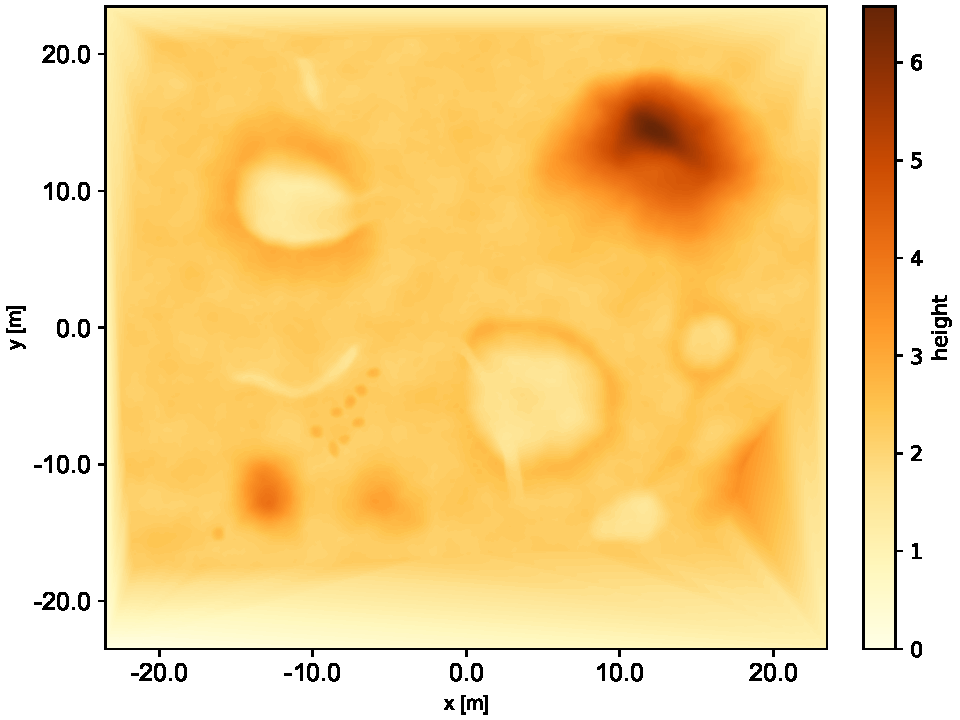
\includegraphics[width=0.48\linewidth]{Figures/elevationMap1.pdf}  
	}
	\subfigure[Map 2] {
    	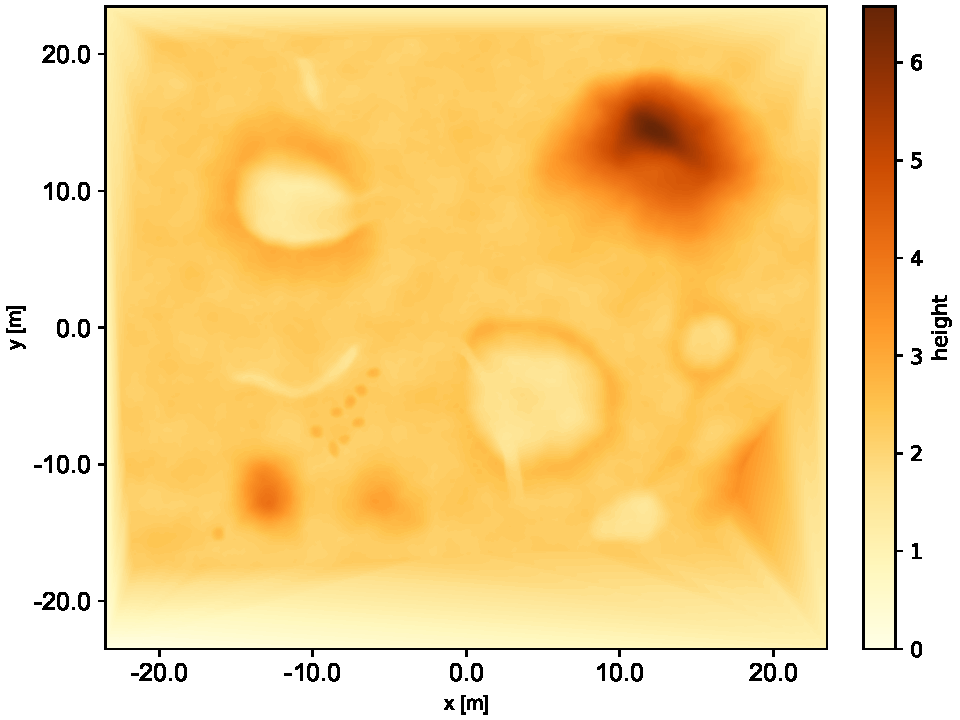
\includegraphics[width=0.48\linewidth]{Figures/elevationMap1.pdf}  
	}
	\end{subfigmatrix}
    \caption{Elevation maps}
    \label{fig:elevationMaps}
\end{figure}

\section{Traversability maps}
\label{section:traversabilityMaps}

\begin{figure}[!ht]
    \centering
	\begin{subfigmatrix}{2}
	\subfigure[Algorithm \ref{alg:slopeMinHeightMap}, where $\yaw = 0$] {
    	\includegraphics[width=0.48\linewidth]{Figures/HeightMinSurface1.pdf}  
	}
	\subfigure[Algorithm \ref{alg:slopeMinHeightMapVarYaw}] {
    	\includegraphics[width=0.48\linewidth]{Figures/HeightMin_maxInclinationSurface1.pdf}  
	}
	\end{subfigmatrix}
    \caption{Traversability maps (case 2; map 1)}
    \label{fig:costMapsCase2Alg2_4}
\end{figure}

\begin{figure}[!ht]
    \centering
	\begin{subfigmatrix}{2}
	\subfigure[Worst-case map] {
    	\includegraphics[width=0.48\linewidth]{Figures/worstCaseSurface1.pdf}  
	}
	\subfigure[Algorithm \ref{alg:refinedMap}] {
    	\includegraphics[width=0.48\linewidth]{Figures/mapRefinementSurface1.pdf}  
	}
	\end{subfigmatrix}
    \caption{Traversability maps (case 2; map 1)}
    \label{fig:costMapsCase2Alg5}
\end{figure} 